\documentclass[../main.tex]{subfiles}
% \hbadness=1000000
% \vbadness=1000000
\begin{document}

\section{Results}
\subsection{The baseline dynamics}
The CA3 and CA1 subregions of the hippocampus exhibit a dynamic interplay between pyramidal cells and specific interneuronal populations, which involves basket and OLM cells in CA3, and basket, OLM, and CCK cells in CA1, giving rise to a characteristic pattern of theta-modulated gamma oscillations.
Figure \ref{fig:baseline-dynamics} illustrates the dynamics of the cyclic network in the CA3 and CA1 subregions, presenting a raster plot that shows the temporal dynamics.
Here, we aligned the theta reference with the firing pattern of the entorhinal cortex layer III (ECIII).
This reference serves as the basis for Figure \ref{fig:phase-spike-distribution} and has been the reference used in the parameter optimization process of the model.
However, for consistency with prevailing literature practices, for the subsequent plots, we transition to using the theta oscillation derived from the local field potential (LFP) measured at the soma stratum (\textit{stratum pyramidale}) in the CA1 subnetwork.
The acativation pattern of the CA1 pyramidal population shows a time lag of approximately 120º or equivalently 42 ms, a temporal shift not solely attributable to network connection delays.
\begin{figure}
    \centering
    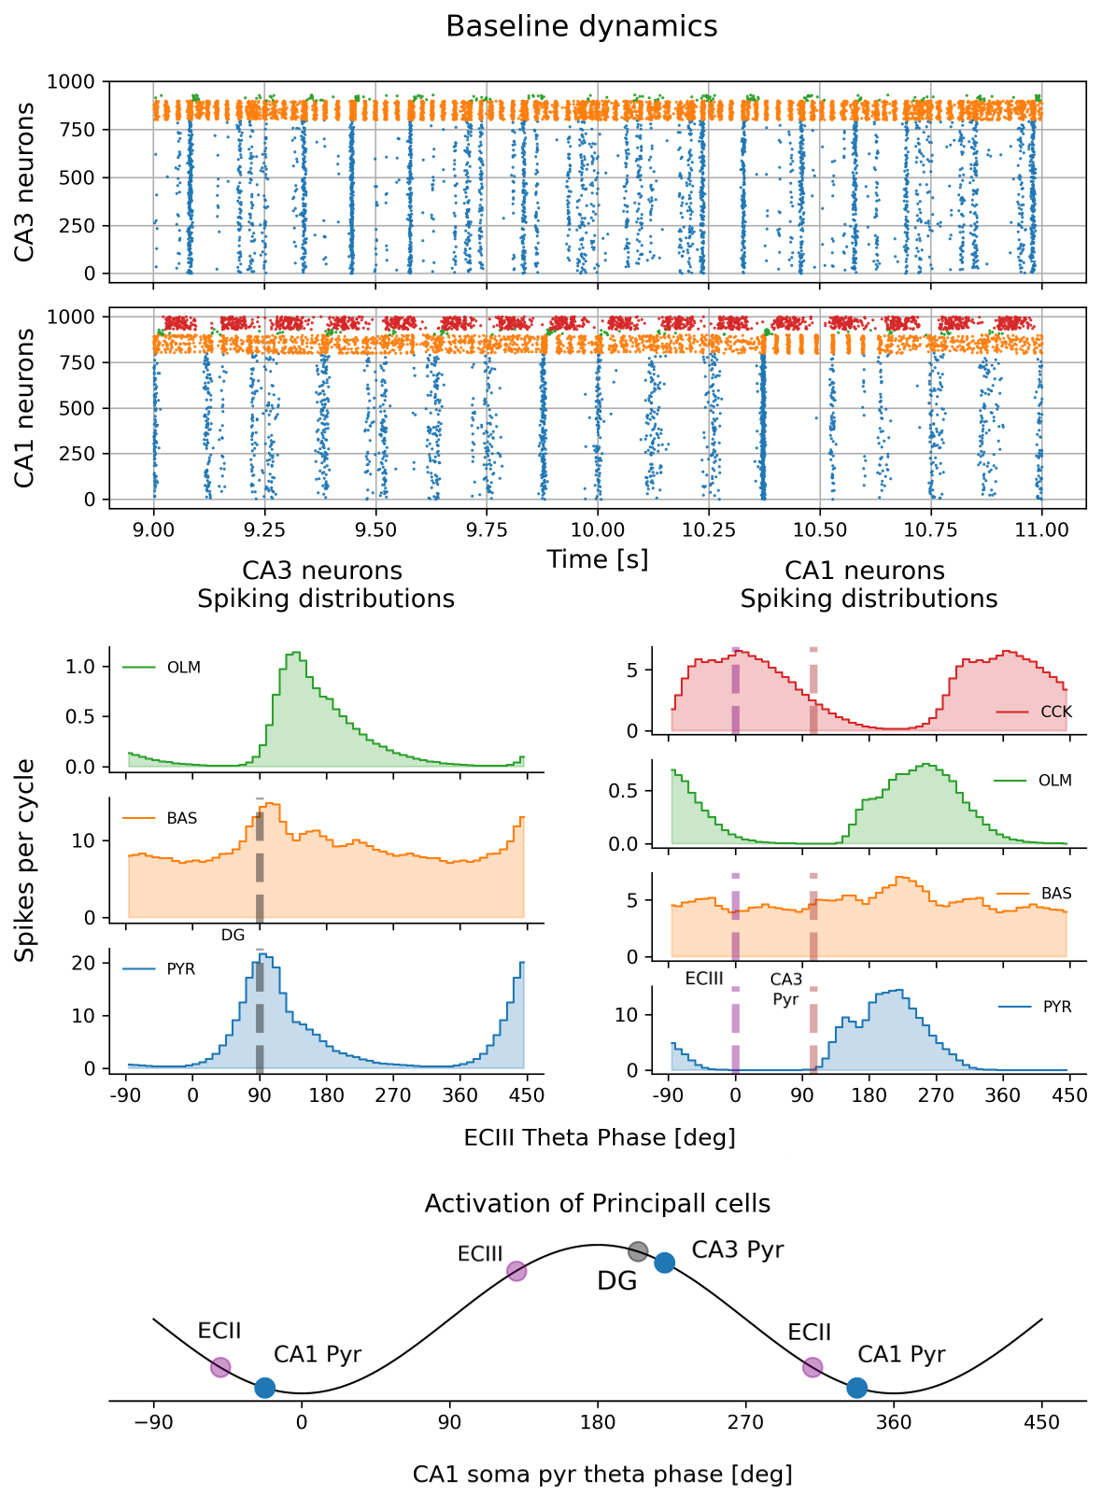
\includegraphics[width=0.9\textwidth]{chapter4/figures/baseline_dynamics-test.png}
    \caption{ \textbf{Baseline dynamics}. Raster plots of CA3 and CA1 subnetworks.Blue, orange, green and red points indicate pyramidal cells, basket cells, olm cells and cck cells, respectively (top).
    Distribution of the number of spikes per cycle over a theta cycle for each category of neurons (medium).
    The theta reference is the one obtained by the external inputs of ECII.
    Gray dashed line indicates the highest level of intensity of the projection from the DG to the basket and pyramidal cells in CA3.
    Purple and brown dashed lines indicate the highest level of intensity of the projections from CA3 (pyramidal cells) and ECII to CCK, basket and pyramidal cells in CA1 subnetwork.
    Activation phase over the CA1 soma pyr theta component of the pyramidal cells and the external inputs (bottom).}
    \label{fig:baseline-dynamics}
\end{figure}
\subsubsection{The cyclic network dynamics}
Within the CA3 subnetwork, pyramidal neurons exhibit influence on OLM and basket neurons through AMPA and NMDA synapses.
Periodically, OLM neurons modulate inhibition in the distal dendrites (Adend3 compartment) of pyramidal neurons, while basket neurons inhibit the the soma.
The interaction between basket cells and pyramidal neurons, operating via the PING mechanism, orchestrates gamma oscillations (at 40 Hz frequency peak in CA3 and 36 Hz frequency peak in CA1), whereas OLM induces a slower modulation in pyramidal neuron activity.

At the same time, this circuit receives synaptic inputs from different sources, including the medial septum (MS), the entorhinal cortex layer II (ECII), and the dentate gyrus (DG), contributing to the various theta oscillations observed within this network segment.
DG inputs, consisting in two subpopulations known as burst and regular, play a pivotal role in imposing specific firing phases on pyramidal cells, influencing the posterior activation timing of OLM cells.

The initiation of pyramidal neuron firing triggered by DG inputs leads to mutual coupling between basket and pyramidal cells, facilitating the generation of gamma oscillations in the network.
MS inputs, originating from two antiphase-firing subpopulations, project onto both the basket cells and the OLM cells.
MS inhibition in OLM cells results in disinhibition of the distal dendrites of pyramidal neurons (Adend3 compartment).

Finally, the ECII inputs, received by both basket and pyramidal neurons in their distal dendrites, maintain the latter in an excited state below their activation threshold.
This setup ensures that once the inputs from the DG arrive, pyramidal neurons start firing, minimizing the response time they would otherwise have on their own.

In the CA1 subnetwork, CCK neurons primarily targets pyramidal neurons in the soma and central dendritic compartment (Adend2) through GABA$_\text{A}$ synapses.
While this inclusion adds complexity to the network, it significantly contributes to the desired activation pattern and enhances theta-gamma coupling.
Synthetic inputs in the CA1 subnetwork include MS inhibition, projected similarly to basket, OLM, and CCK interneurons, along with excitation from ECIII, which stimulates both basket cells and pyramidal neurons (Adend3).
Additionally, it receives inputs from CA3 (Schaffer collateral pathway), conveying information to basket cells, CCK cells, and pyramidal neurons (Adend1).

Upon receiving inputs from CA3, pyramidal neurons in CA1 undergo hyperpolarization, inhibiting these inputs from effectively depolarizing them for firing.
This hyperpolarization is driven by the active CCK cells, stimulated by both ECIII and CA3 excitation.
As CCK cell depolarization subsides, pyramidal neurons begin depolarizing and subsequently generate spikes.
This mechanism results in a significant lag between the populations of pyramidal neurons in CA3 and CA1.

Similar to the CA3 subcircuit, the PING mechanism operates within the activation window of pyramidal neurons, initiating gamma oscillations across the network. Concurrently, OLM neurons are activated, inhibiting the distal dendrites of pyramidal neurons (Adend3), consistent with their role in the CA3 subcircuit.
\subsubsection{Gamma-theta phase-amplitude coupling}
\begin{figure}[t]
    \centering
    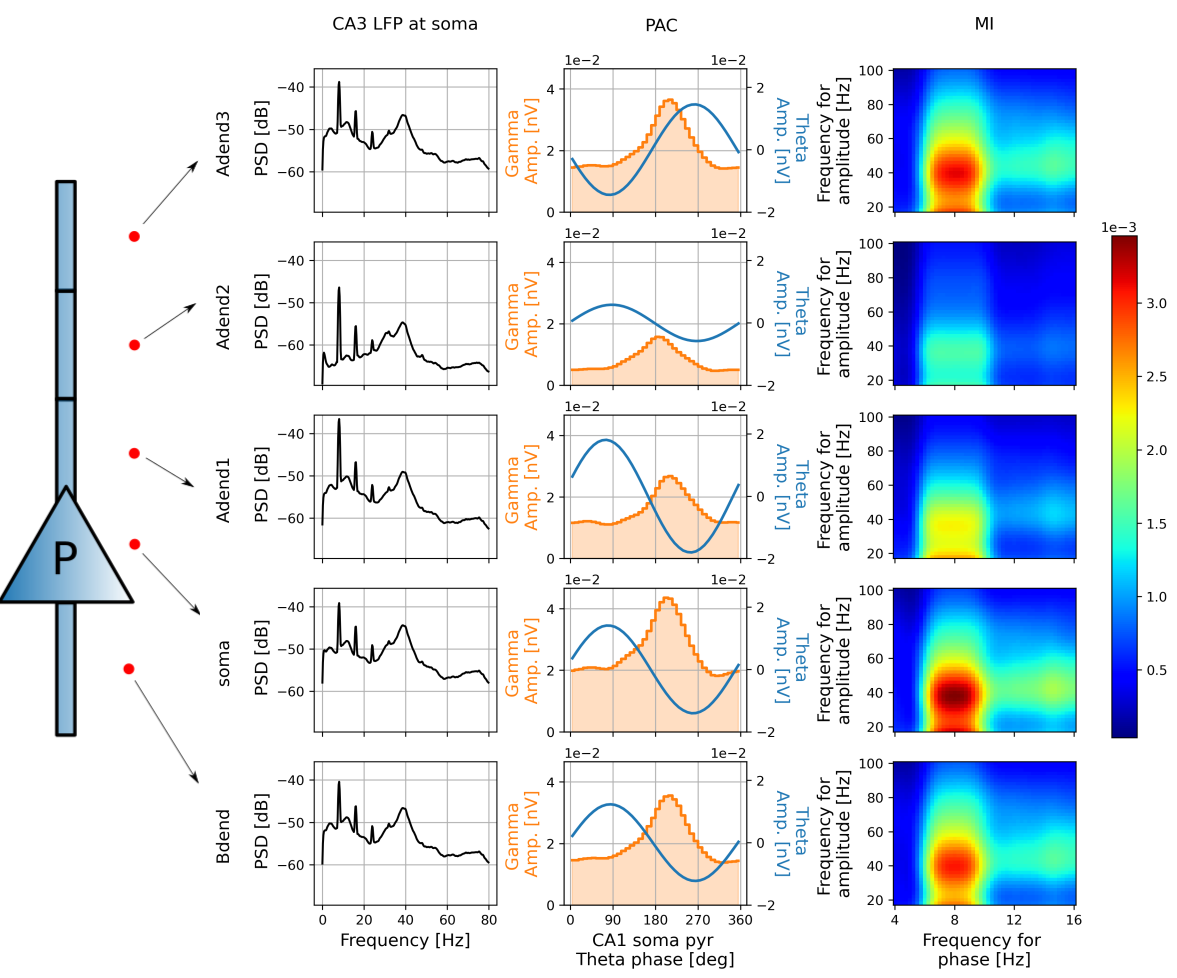
\includegraphics[width=\textwidth]{chapter4/figures/baseline_CA3_properties.png}
    \caption{\textbf{Gamma-theta cross-frequency coupling in each strate of the CA3 subnetwork}: power spectral density (left column), gamma modulated amplitude (center column), and modulation index (right column) of the LFP measured in each strate.
    Theta reference for computing PAC correspond to the theta component of the LFP measured at soma stratum in the CA1 subnetwork.}
    \label{fig:baseline-CA3-properties}
\end{figure}
\begin{figure}[t]
    \centering
    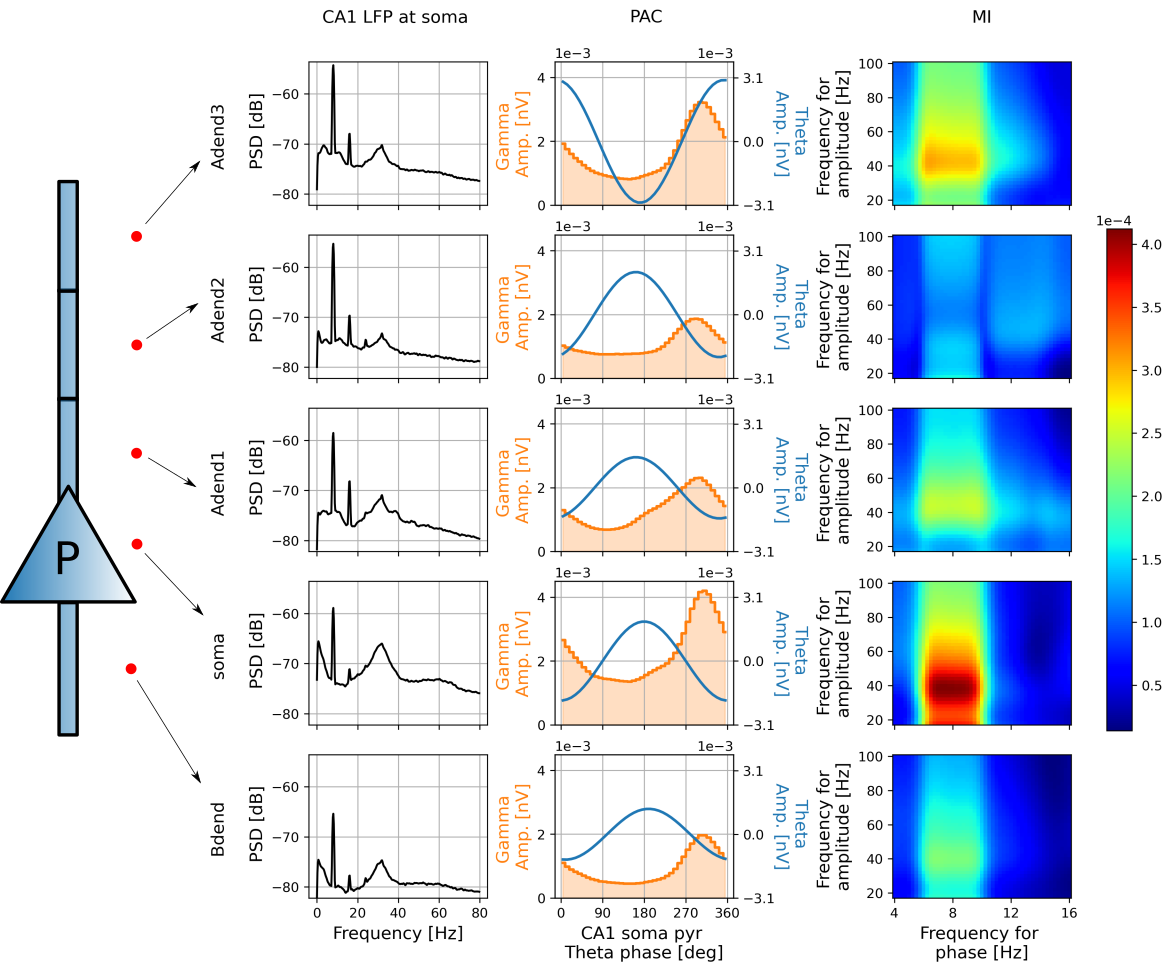
\includegraphics[width=\textwidth]{chapter4/figures/baseline_CA1_properties.png}
    \caption{\textbf{Gamma-theta cross-frequency coupling in each strate of the CA1 subnetwork}: power spectral density (left column), gamma modulated amplitude (center column), and modulation index (right column) of the LFP measured in each strate.
    Theta reference for computing PAC correspond to the theta component of the LFP measured at soma stratum in the CA1 subnetwork.}
    \label{fig:baseline-CA1-properties}
\end{figure}
Figures \ref{fig:baseline-CA3-properties} and \ref{fig:baseline-CA1-properties} illustrate the power spectral density (PSD) of the Local Field Potentials (LFPs) and theta-gamma phase-amplitude coupling (PAC) measurements for the CA3 and CA1 subnetworks.
LFPs were computed across each stratum or layer where each compartment is placed.

The PSD reveals the presence of theta and gamma bands in each stratum or layer.
Theta, characterized by a narrow peak at 8 Hz, and the broader gamma band, peaking at 40 Hz in CA3 and 35 Hz in CA1.
Power variations within strata are observed due to distinct interactions.
The Adend1 stratum notably exhibits a stronger theta peak, attributed to excitatory inputs from the DG, serving as the primary driver for pyramidal cells.
Conversely, the soma stratum demonstrates higher gamma band power, predominantly influenced by continuous inhibition from basket cells.
Additionally, the Adend3 stratum displays notable theta peak amplitude due to the influence of OLM neuron-mediated inhibition.

Theta-gamma CFC was computed by two methods: by quantifying the gamma oscillation amplitude concerning the theta cycle (PAC) and by the modulation index (MI). 
Both approaches offer complementary insights, with the MI delineating the frequency ranges with pronounced coupling and the former illustrating modulation phase and efficacy concerning the theta cycle.
The difference between minimum and maximum gamma amplitude, usually labeled as $h$ \citep{kramer2016case}, correlates with the modulation index, emphasizing the efficacy of modulation in the theta cycle.
Enhanced CFC is observed in the soma stratum due to earlier mentioned reasons and in the Adend3 stratum owing to potent theta component power from OLM inhibition.
This phenomenon is consistent across both subnetworks, except for the Bdend stratum, where CA3 demonstrates higher coupling, attributed to autoexcitation present in CA3 pyramidal neurons, absent in CA1.

An insightful aspect revealed by the model involves the interrelationship among diverse theta components within different strata.
Considering the theta oscillation peak in the soma stratum as a reference point, we observed a minor lead in Adend1 and a more pronounced one in Adend2.
Conversely, in the Adend3 stratum, the theta oscillation demonstrates antiphase behavior respect to the soma stratum.
This discrepancy results from intricate interactions involving entorhinal cortex (EC) inputs, inhibitory influences by OLM cells, and intradendritic currents.
Notably, the self-excitation of pyramidal cells contributes to the phase alignment of theta components between the soma and Bdend strata in CA3, while in CA1, a slight delay is observed in the latter.
This connection enhances not only coherence among theta components but also promotes gamma-theta coupling within this stratum.

Furthermore, another difference between the CA1 and CA3 subnetworks emerges in the amplitude of the theta component within the Adend2 stratum.
While in CA3, its amplitude is comparatively lower due to the absence of synaptic projections, periodic inhibition from CCK neurons in CA1 enhances the amplitude of theta oscillations within this stratum.

Regarding gamma oscillations, the phase exhibiting the highest amplitude aligns with the activation phase of pyramidal neurons, coinciding with the moment of PING mechanism occurrence within the theta cycle, ocurring at the descending phase of the theta cycle.
This consistent activation phase is observed across all LFP measurement strata due to intradendritic transmission between compartments within pyramidal neurons in our model.
However, the amplitude variations across strata are attributable to distinct interactions specific to each.

\subsection{The role of CCK neurons}
As earlier mentioned, the CCK population determine the firing phase of the pyramidal neurons. 
Theoretically, considering the phase of external inputs arriving at the CA1 region, the experimentally observed phase difference greater than half a theta cycle between the populations of pyramidal neurons in CA3 and CA1 cannot be explained solely by axonal propagation and neuronal response dynamics.

The existence of at least a third interneuron is essential to elucidate this phase discrepancy.
This suggests that local inhibition by interneurons, specifically targeting pyramidal neurons, plays a crucial role in establishing and modulating the observed phase differences, surpassing the anticipated impact of axonal propagation and neuronal response dynamics alone \citep{mizuseki_theta_2009,cutsuridis_computational_2015}.
\begin{figure}[!htb]
    \centering
    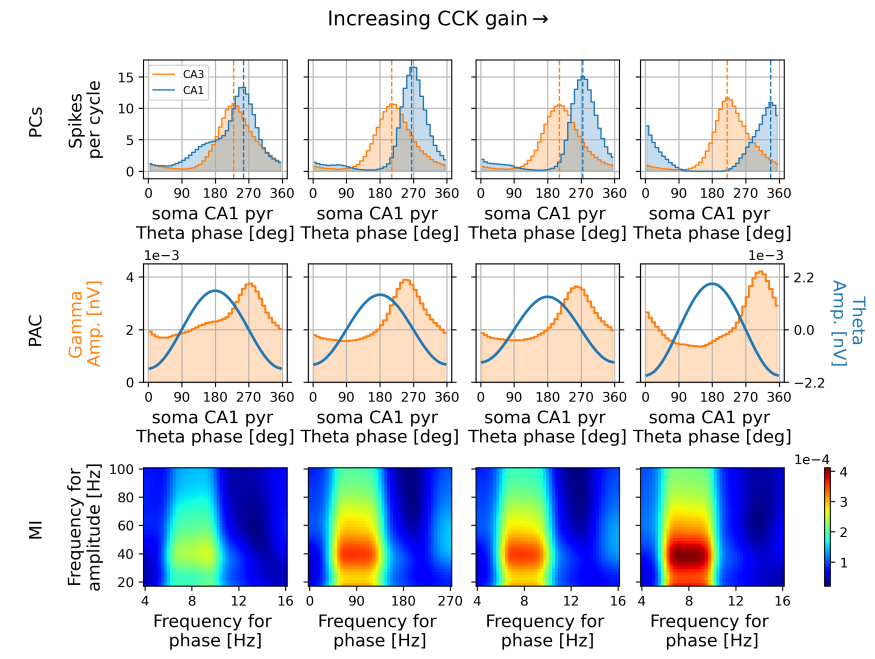
\includegraphics[width=\textwidth]{chapter4/figures/cckCA1_gain.png}
    \caption{\textbf{CCK inhibition into the CA1 subfield}.
    From left to right, the level of inhibition is increased until reach the baseline state.
    From top to bottom: distribution of pyramidal cells spikes per theta cycle,
    gamma modulated amplitude over theta cycle and modulation index.
    Dashed lines in the distributions indicate the maximum probability of spikes of each pyramidal population.}
    \label{fig:cck-gain}
\end{figure}

Our proposal has been the addition of the non-basket CCK cells as third type of interneuron population.
CCK cells, are known for their role in mediating feedforward inhibition onto CA1 pyramidal neuron dendrites, and play a pivotal role in regulating the activity of these neurons in response to ECIII inputs.
Their location around the border between the \textit{stratum radiatum} and \textit{stratum lacunosum-moleculare} in the CA1 hippocampal region enables them to receive excitatory inputs from the ECIII and respond by spiking, which suggest their involvement in modulating CA1 pyramidal neuron activity triggered by ECIII inputs \citep{bilash_lateral_2023}.
Considering the intricate involvement of CCK cells in regulating dendritic activity and integrating cortical inputs, their inclusion in the CA1 hippocampal model is fundamental make them a good candidate for accurately reproduce the specific patterns of activation among pyramidal cells cycle by cycle.

\begin{figure}[htbp]
    \centering
    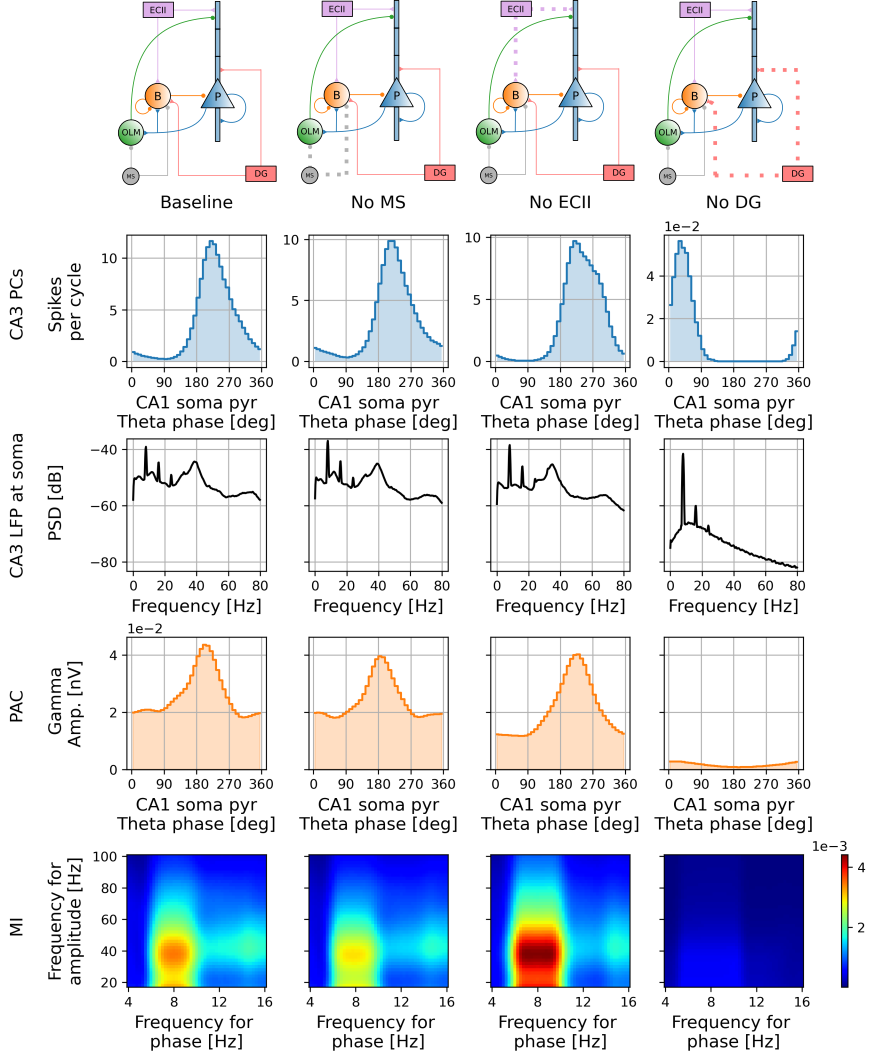
\includegraphics[width=\textwidth]{chapter4/figures/removing_external_inputs/removing_inputs_ca3_lfp.png}
    \caption{\textbf{Effect of external input removal on CA3 subnetwork dynamics}.
    From top to bottom: Distribution of spikes per theta cycle of pyramidal neurons, power spectral density  of the soma LFP, phase-amplitude coupling between theta and gamma filtered soma LFP, and modulation index of the soma LFP.
    From left to right: Baseline state, removal of MS inputs, removal of ECII inputs and removal of DG inputs.
    Note that the scale is shared in each column excepting in the distribution plots.}
    \label{fig:no-inputs-ca3}
\end{figure}
The increase in inhibition from CCK neurons to pyramidal neuron, as depicted in Figure \ref{fig:cck-gain}, correlates with a progressive rise in the phase discrepancy between CA3 and CA1 pyramidal neurons, eventually aligning with the desired firing phase observed in the baseline state.
Moreover, this heightened inhibition triggers an escalation in the cross-frequency coupling of the LFP, as measured by the utilized metrics.
\subsection{The role of the external inputs}
\begin{figure}[!htb]
    \centering
    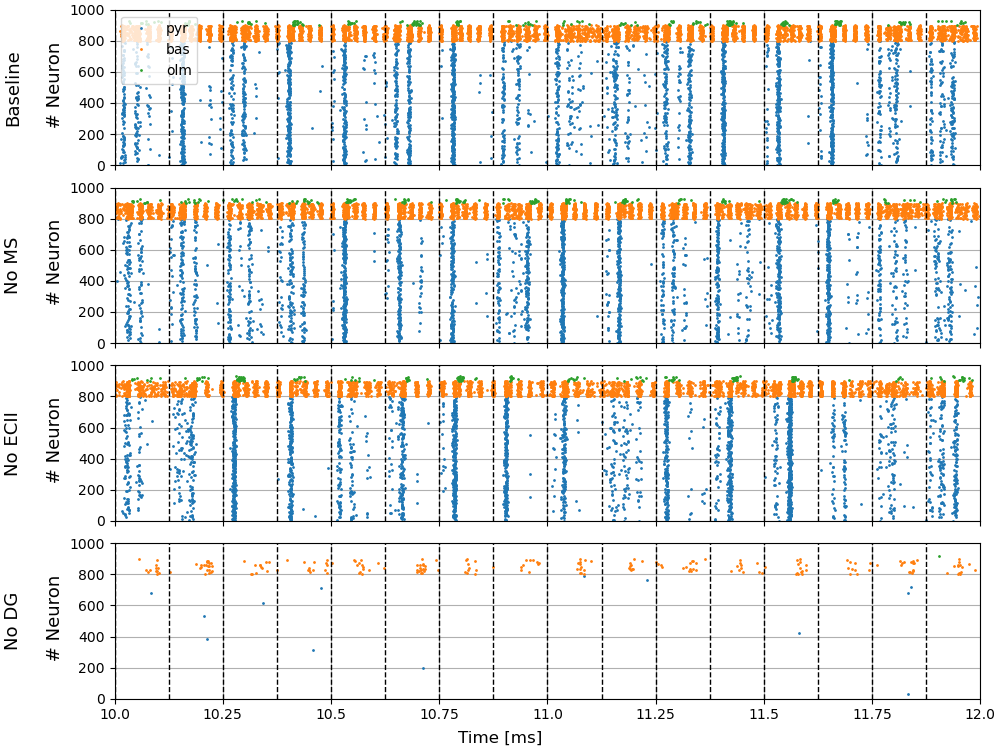
\includegraphics[width=\textwidth]{chapter4/figures/removing_external_inputs/removing_inputs_ca3_rasters.png}
    \caption{\textbf{Effect of external input removal in the CA3 subnetwork dynamics}.
    From top to bottom, the raster plots of the baseline state, the state of removing MS inputs, the state of removing ECII inputs and state of removing DG inputs.
    Blue, orange and green colors indicate pyramidal, basket and OLM cells, respectively.}
    \label{fig:inputs-ca3-rasters}
\end{figure}
\begin{figure}[!htb]
    \centering
    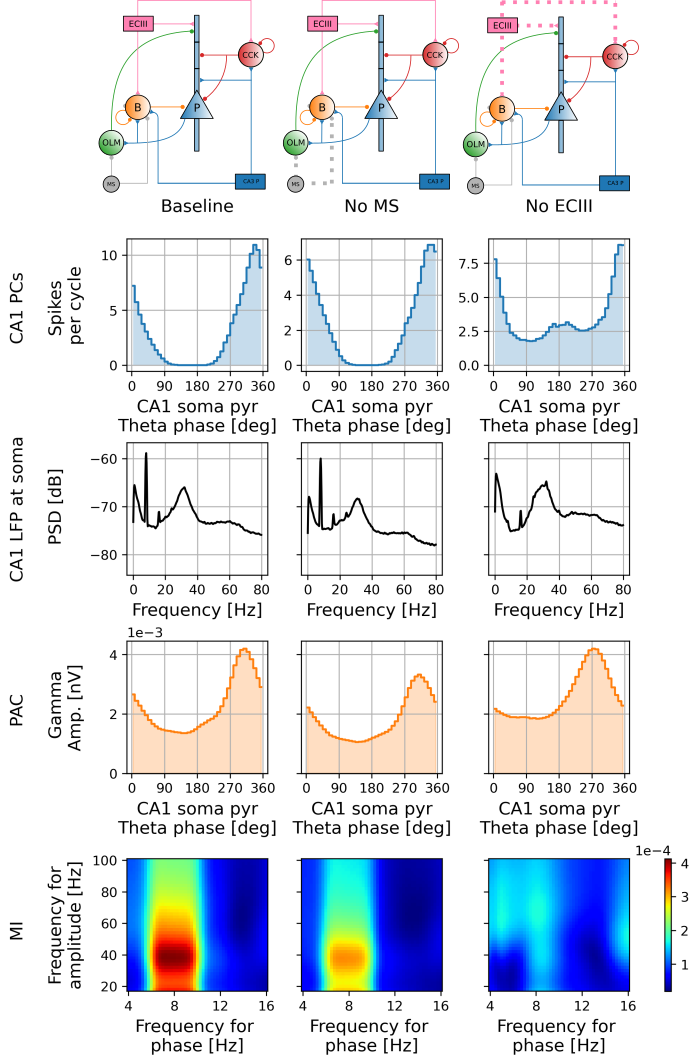
\includegraphics[width=0.75\textwidth]{chapter4/figures/removing_external_inputs/removing_inputs_lfp_ca1_pt1.png}
    \caption{\textbf{Effect of external input removal on CA1 subnetwork dynamics}.
    From top to bottom: Distribution of spikes per theta cycle of pyramidal neurons, power spectral density of the soma LFP, phase-amplitude coupling between theta and gamma components of soma LFP, and the modulation index of the soma LFP.
    From left to right: Baseline state, removal of MS 
    inputs, and removal of ECIII inputs.
    Note that the scale is shared in each row excepting in the distribution plots.}
    \label{fig:no-inputs-ca1}
\end{figure}
\begin{figure}[htbp]
    \ContinuedFloat % To indicate continuation of the previous table
    \centering
    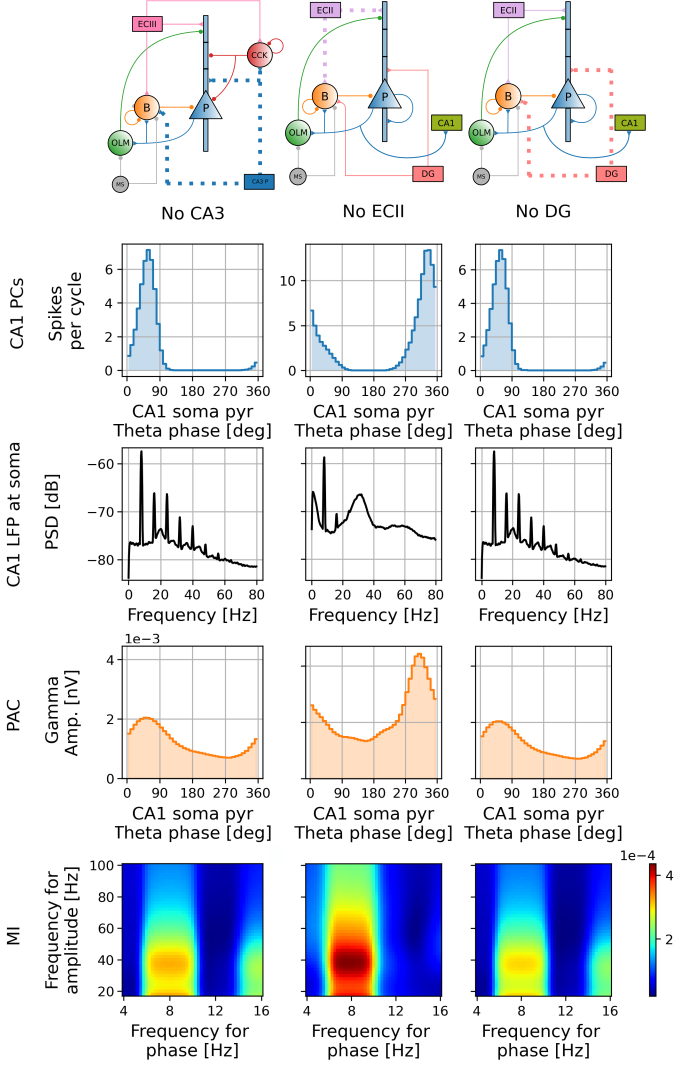
\includegraphics[width=0.75\textwidth]{chapter4/figures/removing_external_inputs/removing_inputs_lfp_ca1_pt2.png}
    \caption{\textbf{Effect of external input removal on CA1 subnetwork dynamics (continuation).}.  
    From left to right: Removal of the CA3 inputs generated by the CA3 subnetwork, removal of ECIII inputs, removal of DG }
    % \label{fig:no-inputs-ca1}
\end{figure}
% rasters CA1 removing external inputs
\begin{figure}[htbp]
    \centering    
    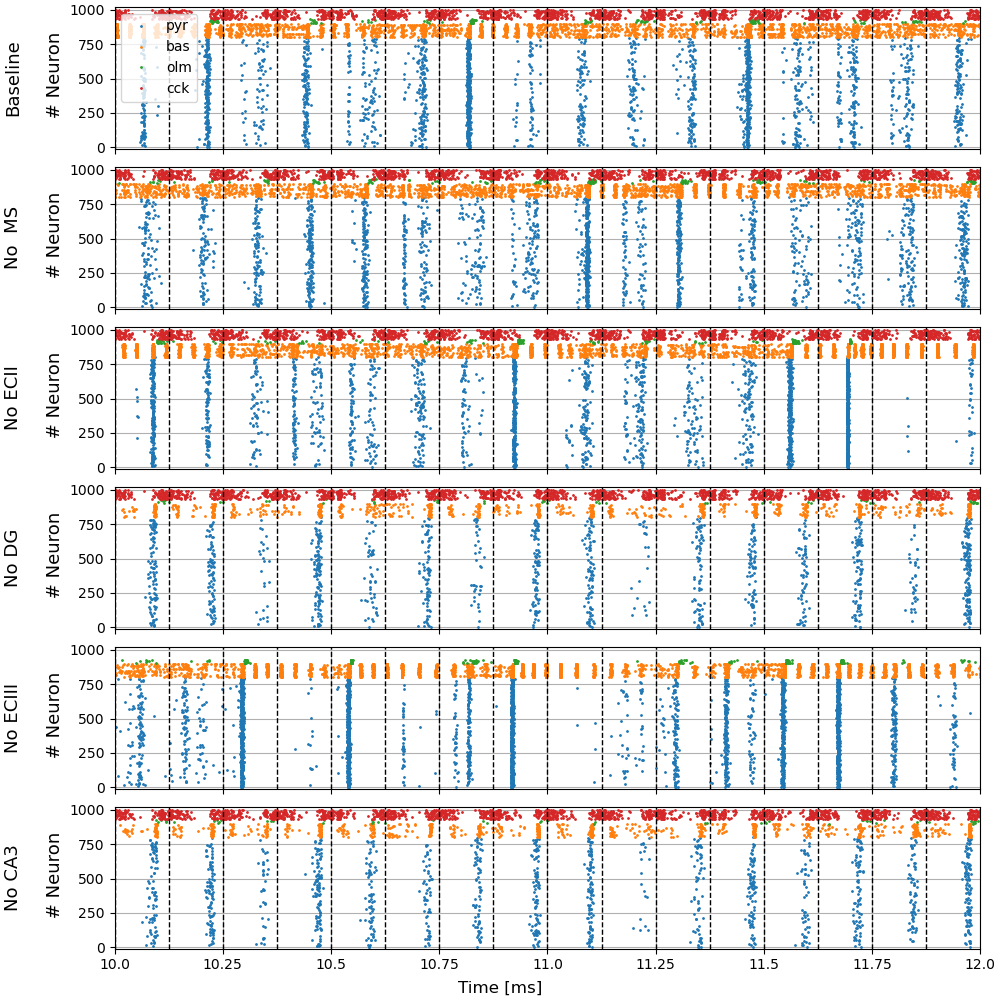
\includegraphics[width=\textwidth]{chapter4/figures/removing_external_inputs/removing_inputs_ca1_rasters.png}
    \caption{\textbf{Effect of external inputs removal in the CA1 subnetwork dynamics}.
    From top to bottom, the raster plots of the baseline state, the state of removing MS inputs, the state of removing ECII inputs, the state of removing DG inputs, the state of removing ECIII inputs, and the state of removing CA3 inputs generated by the CA3 subnetwork.
    Blue, orange and green colors indicate pyramidal, basket and OLM cells, respectively.}
    \label{fig:inputs-ca1-rasters}
\end{figure}
The effects of each kind of input within the network exhibit distinctive effect on the emergent dynamics of the model.
Figures \ref{fig:no-inputs-ca3} and \ref{fig:no-inputs-ca1} illustrate the effect of removing each specific input within the CA3 and CA1 subnetwork, respectively, presenting spiking distributions across the theta cycle, power spectral density of the LFP, and phase-amplitude coupling measured by the theta-modulated gamma-amplitude and the modulation index.
Figures \ref{fig:inputs-ca3-rasters} and \ref{fig:inputs-ca1-rasters} shows the corresponding raster plots of each scenario in the CA3 and CA1 subntetwork, respectively. 

When MS inputs are removed, both the CA3 and CA1 networks maintain a similar cyclic pattern but with reduced cross-frequency coupling compared to the baseline state.
Conversely, the removal of EC inputs in either CA3 or CA1 subnetworks increases cross-frequency coupling.
Hence, each of these theta sources distinctly influences the coupling of theta and gamma rhythms, a phenomenon that will be further analysed.

The DG inputs hold a significantly different role in the network.
Despite being a crucial theta source, they primarily act as the principal driver of the network.
When DG inputs are absent, CA3 pyramidal neurons exhibit minimal spiking, leading to the cessation of gamma oscillations.
This absence of DG inputs prevents pyramidal cells from reaching the activation threshold, resulting in the absence of gamma oscillations.
% (Figures \ref{a-fig:inputs-ca3-rasters} and \ref{a-fig:inputs-ca3-lfps}).
In turn, CA1 pyramidal neurons continue exhibiting activity due to background noise.
However, the lack of excitation of basket cells, driven by CA3 pyramidal neuron synapses, significantly reduces gamma oscillations.
% (Figures \ref{a-fig:inputs-ca1-rasters} and \ref{a-fig:inputs-ca1-lfps}).

In the CA1 subnetwork, the removal of ECIII inputs prevents CCK neurons from depolarizing enough to spike, resulting in no inhibition to pyramidal neurons.
Consequently, the activation of pyramidal neurons in CA1 synchronizes with CA3 pyramidal neurons, reducing the expected time lag.
Simultaneously, the theta-gamma coupling significantly decreases. 
In the PSD, the frequency peak at 8Hz dissapears, highlighting the importance of this input for the proper coupling between different theta sources in the network.
% \textcolor{blue}{Raster plots and LFPs for each discussed scenario are depicted in Figures \ref{a-fig:inputs-ca3-rasters}, \ref{a-fig:inputs-ca3-lfps} and Figures \ref{a-fig:inputs-ca1-rasters},\ref{a-fig:inputs-ca1-lfps} for CA3 and CA1 subnetworks, respectively.}
\subsubsection{ECII excitation worsens the cross-frequency coupling}
Figure \ref{fig:no-ec2-input-ca3} illustrates a comparative between these effects observed upon the removal of the ECII and the MS inputs in relation to the CA3 network baseline state.
It displays various measurements for both the theta and gamma components of the LFP in the soma stratum, including the power of the PSD, amplitude of the maximum, frequency of the maximum, and standard deviation of the cycle duration for each component (left). 
Notably, the measure of gamma oscillation has been calculated with respect to the envelope. 
Additionally, the distribution of gamma band frequencies over the phases of the theta component is depicted (right).
\begin{figure}[!htb]
    \centering
    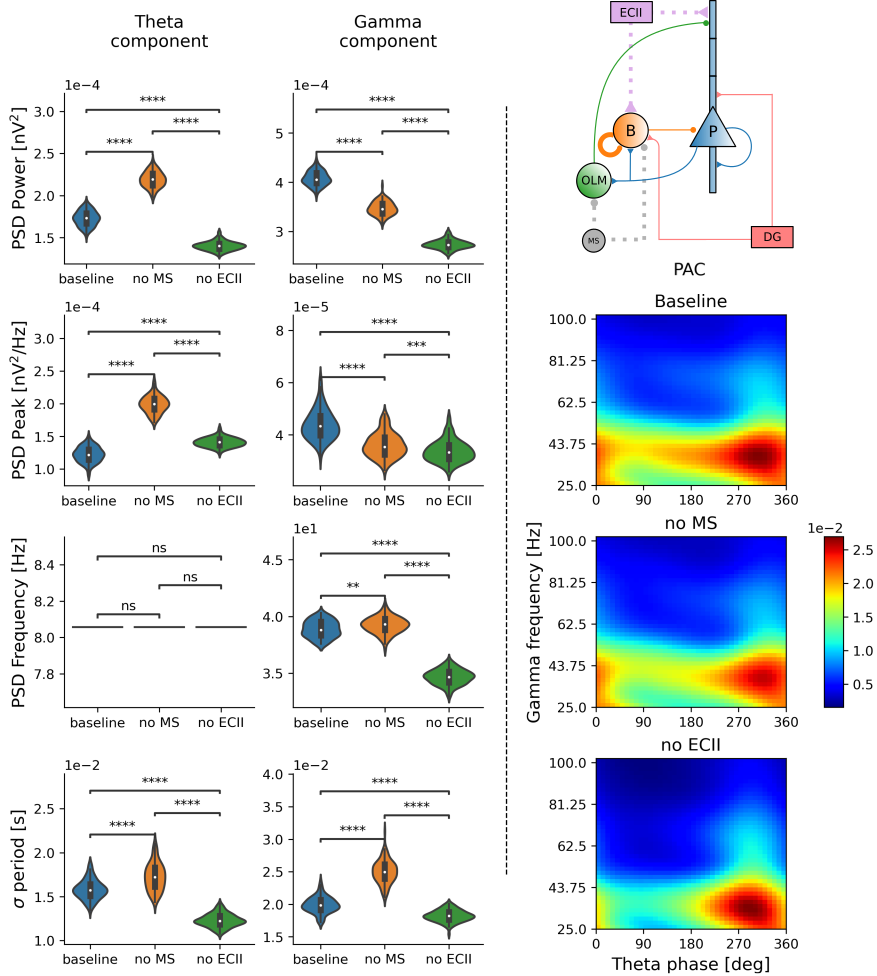
\includegraphics[width=\textwidth]{chapter4/figures/no_ec2_ms_inputs_ca3.png}
    \caption{\textbf{Effect of ECII and MS input removal  CA3 subnetwork dynamics}.
    Left panels shows the PSD power, the PSD peak, the PSD frequency and the standard deviation of the period of theta and gamma oscillations.
    Right panels shows the distribution of the gamma frequencies over the phases of the theta rythm of 8 Hz, the theta oscillation of the network.
    We used Mann-Whitney U test to determine statistical significance between the means, and followed the criteria where ns: p > 0.05, *: p $\leq$ 0.05, **: p $\leq$ 0.01,***: p $\leq$ 0.001, ****: p $\leq$ 0.0001.}
    \label{fig:no-ec2-input-ca3}
\end{figure}
The ECII input targets both basket cells and pyramidal cells in the Adend3 layer.
As discussed earlier, DG inputs predominantly drive pyramidal cells, maintaining an in-phase relationship with them. Consequently, in isolated pyramidal cell populations, the ECII input exhibits no discernible impact on their spiking dynamics. In basket cells, these ECII excitatory inputs contribute significantly to the generation of gamma oscillations.
These inputs are received through AMPA and NMDA synapses.
The latter, due to their longer decay constants, do not have an important modulatory effect like AMPA but rather a net effect resembling a constant current.
Therefore, the removal of this input results in a lower population frequency of basket cells (35Hz), due to the absence of the NMDA excitation.
Simultaneously, the theta oscillation, interacting with various other oscillations, experiences alterations.
This includes those generated by MS inputs, DG inputs, and the oscillation transmitted by pyramidal neurons, ultimately generated by DG inputs arrival at Adend1 stratum.

Within pyramidal neurons, there is a filtering process from distal dendrites to soma, where basket cells projections are placed.
Consequently, both basket and pyramidal elements are less excited following the removal of this input, with pyramidal neurons being less affected than basket cells compared to the baseline configuration.
Consequently, the removal of ECII input results in a net effect on basket-pyramidal coupling, leading to an increase in cross-frequency coupling. 
The resultant theta oscillation becomes more stable, displaying a larger peak amplitude and more regular cycles, facilitating improved coupling of gamma oscillations. 
In other words, the amplitude of gamma oscillations is distributed across fewer phases of the theta cycle compared to the baseline, as it can be observed.
\clearpage
\subsubsection{MS inhibition enhances the cross-frequency coupling}
The opposite effect has been observed with inputs from the MS.
Unlike the situation with ECII inputs, removing the MS inputs result into a decrease in cross-frequency coupling.
Similar to the removal of ECII inputs, there is no significant change in the activation pattern of pyramidal neurons.
Although the change in the dominant frequency of the gamma band is significant, the increase is small in relative terms.
The decrease in cross-frequency coupling implies that the amplitude of gamma oscillations is more evenly distributed over the phases of the theta cycle.
This is because the role of the MS input is to synchronize the gamma oscillations that emerge from the basket-pyramidal interaction (PING).
In other words, MS inputs act as a clock on the basket cells, providing stability to the set of gamma oscillations generated in each cycle.
By removing this clock, gamma oscillations become more disorganized and unstable.
Therefore, while \textbf{ECII input weakens the stability of the emerging theta oscillation}, \textbf{the inhibition of MS inputs organizes gamma oscillations} concerning the theta component.

Although this analysis was conducted in the CA3 network, the same conclusions can be drawn for the CA1 network, where the role of ECII inputs is played by ECIII inputs.
% \textcolor{blue}{In Appendix 3, Figures \rf{a-fig:inputs-ca3-rasters},\ref{a-fig:inputs-ca1-rasters} shows examples of the rasters plots of each configuration generated by inhibitory supression.
% In the same way, Figures \ref{a-fig:inputs-ca3-lfps},\ref{a-fig:inputs-ca1-lfps} show the theta- and gamma-filterted LFP measured at the soma stratum.}

\subsection{The effect of interneuron inhibition in the network}
Figures \ref{fig:no-inhibition-ca3} and \ref{fig:no-inhibition-ca1-1} provide a comparison between the baseline state and the condition post-removal of CA3 local inhibitory connections.
This comparison evaluates the activation pattern of pyramidal cells and the phase-amplitude coupling of the LFP at the soma stratum.
Additionally, Figures \ref{fig:interneurons-ca3-rasters} and \ref{fig:interneurons-ca1-1-rasters} illustrate the correspoding raster plots of CA3 and CA1 subnetwork dynamics for each condition considered.
\begin{figure}[htbp]
    \centering
    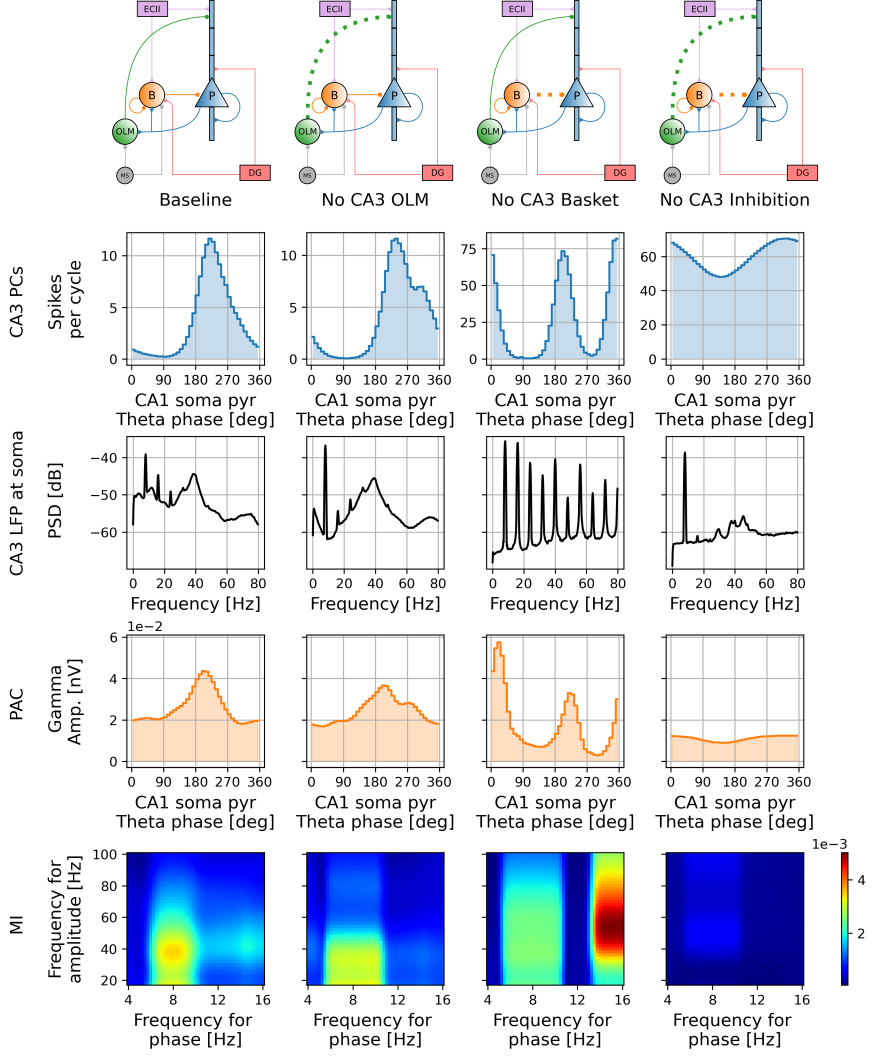
\includegraphics[width=\textwidth]{chapter4/figures/removing_interneurons/removing_interneurons_ca3_lfp.png}
    \caption{\textbf{Effect of interneuron inhibition removal on CA3 subnetwork dynamics}.
    From top to bottom: Distribution of spikes per theta cycle of pyramidal neurons, power spectral density of the soma LFP, phase-amplitude coupling between theta and gamma filtered soma LFP, and modulation index of the soma LFP. 
    From left to right: baseline state, removal of OLM cells projections, removial of basket cells projections, and removal of all interneuron inihibition.
    Note that the scale is shared in each column excepting in the distribution plots.}
    \label{fig:no-inhibition-ca3}
\end{figure}
% rasters CA3 removing inhibition
\begin{figure}[t]
    \centering
    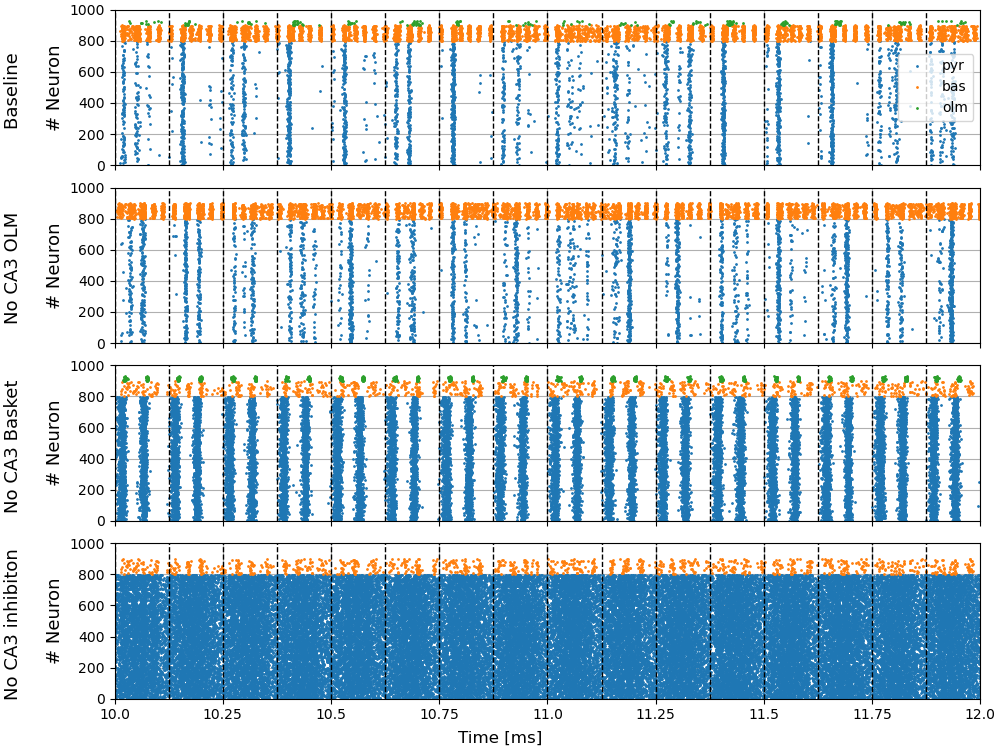
\includegraphics[width=\textwidth]{chapter4/figures/removing_interneurons/removing_interneurons_ca3_rasters.png}
    \caption{\textbf{Effect of interneuron inhibition removal on CA3 subnetwork dynamics}.
    From top to bottom, the raster plots of the baseline state, the state of removing OLM cells projections, the state of removing basket cells projections, and the state of removing the all interneuron inhibition.
    Blue, orange and green colors indicate pyramidal, basket and OLM cells, respectively.}
    \label{fig:interneurons-ca3-rasters}
\end{figure}
The removal of inhibition from OLM cells displays no significant alteration in the activation pattern.
However, it notably decreases theta-gamma coupling, as observed in the modulation index.
Theta oscillations seem more consistent in amplitude, yet the variability in the activation pattern of pyramidal neurons increases.

In contrast, the absence of inhibition from basket cells induces a substantial network state alteration.
This alteration involves dual activation of pyramidal neurons per theta cycle, with a similar activation pattern observed in OLM cells.
Consequently, this dual activation shifts the primary LFP frequency from 8 Hz to 16 Hz, as evident in the peak modulation index observed near this frequency.

Furthermore, a scenario without inhibition from interneurons results in continuous activity of pyramidal neurons throughout the theta cycle, modulated primarily by the DG inputs, leading to increased spike emission in this neuronal population.
% \begin{figure}[htbp]
\begin{figure}[!htbp]
    \centering
    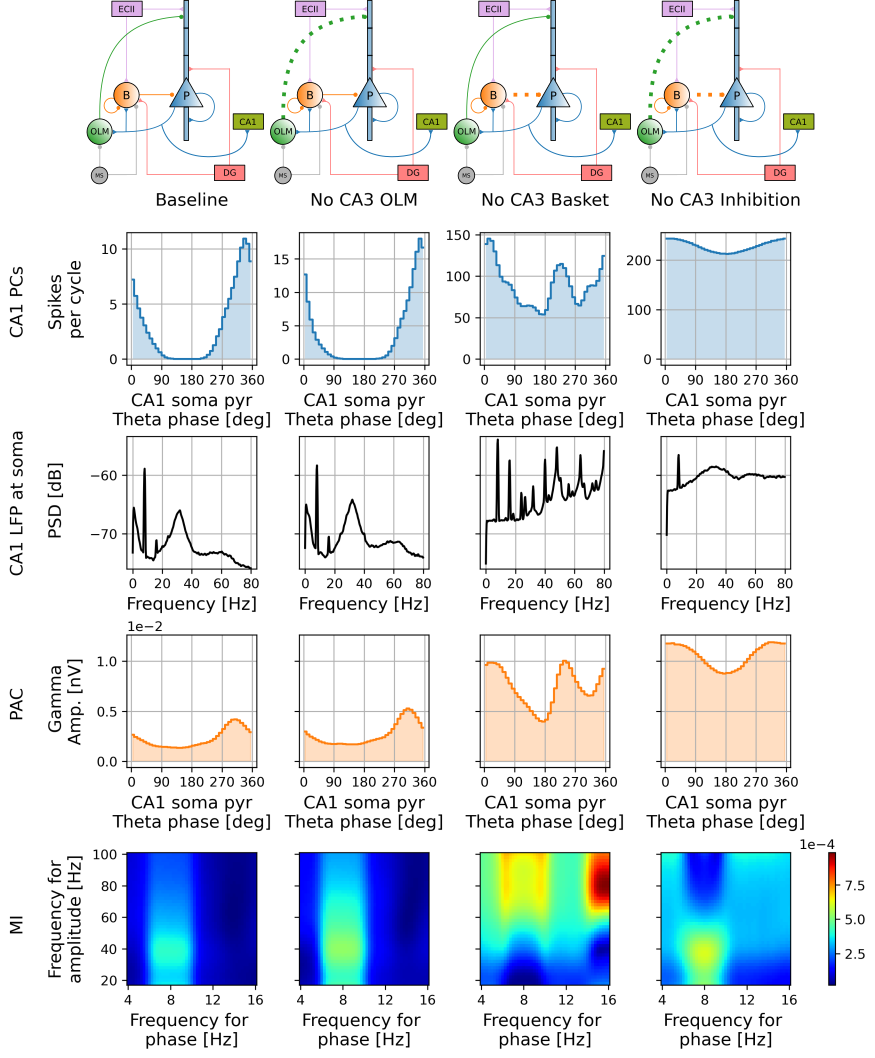
\includegraphics[width=\textwidth]{chapter4/figures/removing_interneurons/removing_interneurons_ca1_v1_lfp.png}
    \caption{\textbf{Effect of CA3 inhibition removal on CA1 subnetwork dynamics}.
    From top to bottom: Distribution of spikes per theta cycle of pyramidal neurons, power spectral density  of the soma LFP, phase-amplitude coupling between theta and gamma filtered soma LFP, and modulation index of the soma LFP.
    From top to bottom: baseline state, removal of CA3 OLM cells projections, removal of CA3 basket cells projections, and removal of all CA3 interneuron inhibition.
    Note that the scale is shared in each column excepting in the distribution plots.}
    \label{fig:no-inhibition-ca1-1}
\end{figure}

\begin{figure}[t]
    \centering
    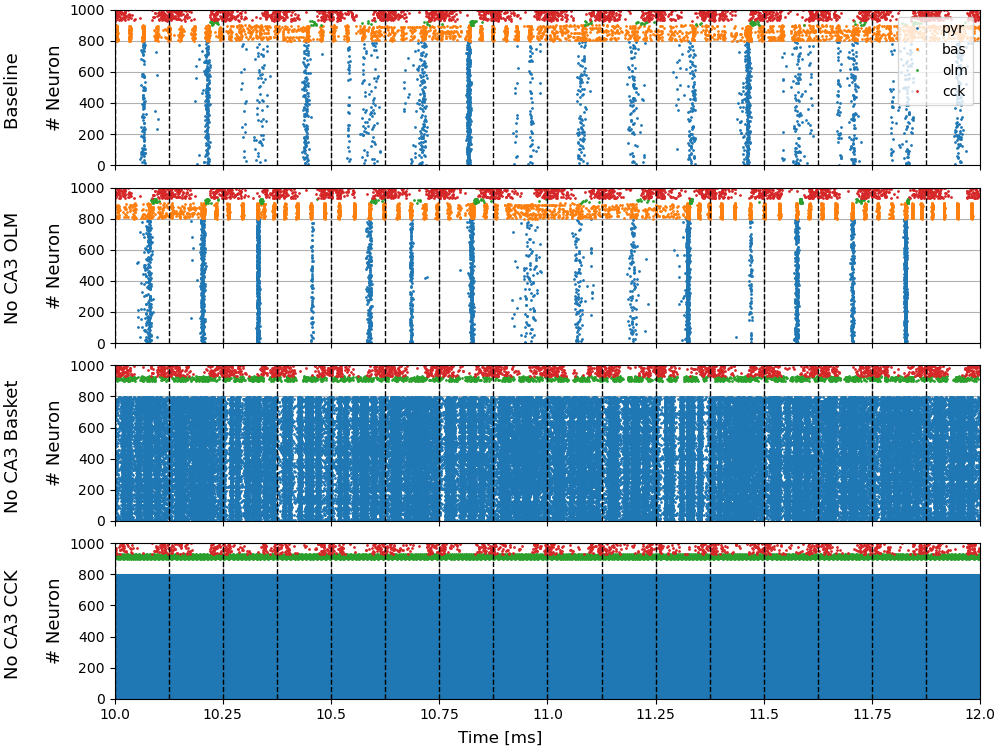
\includegraphics[width=\textwidth]{chapter4/figures/removing_interneurons/removing_interneurons_ca1_v1_rasters.png}
    \caption{\textbf{Effect of CA3 interneuron inhibition removal on CA1 subnetwork dynamics}.
    From top to bottom, the raster plots of the baseline state, the state of removing OLM cells projections, the state of removing basket cells projections, and the state of removing the all interneuron inhibition.
    Blue, orange, green and red colors indicate pyramidal, basket, OLM and CCK cells, respectively.}
    \label{fig:interneurons-ca1-1-rasters}
\end{figure}

On the other hand, Figure \ref{fig:no-inhibition-ca1-2} shows the effects of local inhibition removal within CA1 (Figure \ref{fig:interneurons-ca1-2-rasters} shows the corrsponding raster plots).
Similar to CA3, the reduction of OLM cell inhibition reduces theta-gamma coupling while slightly delaying the peak activation of pyramidal neurons compared to the baseline configuration.
However, unlike the CA3 subnetwork, the absence of basket cell inhibition does not produce a similar activation pattern due to the inhibitory action of CCK neurons, which persist in generating a delayed response to CA3 excitation.
\begin{figure}[htbp]
    \centering
    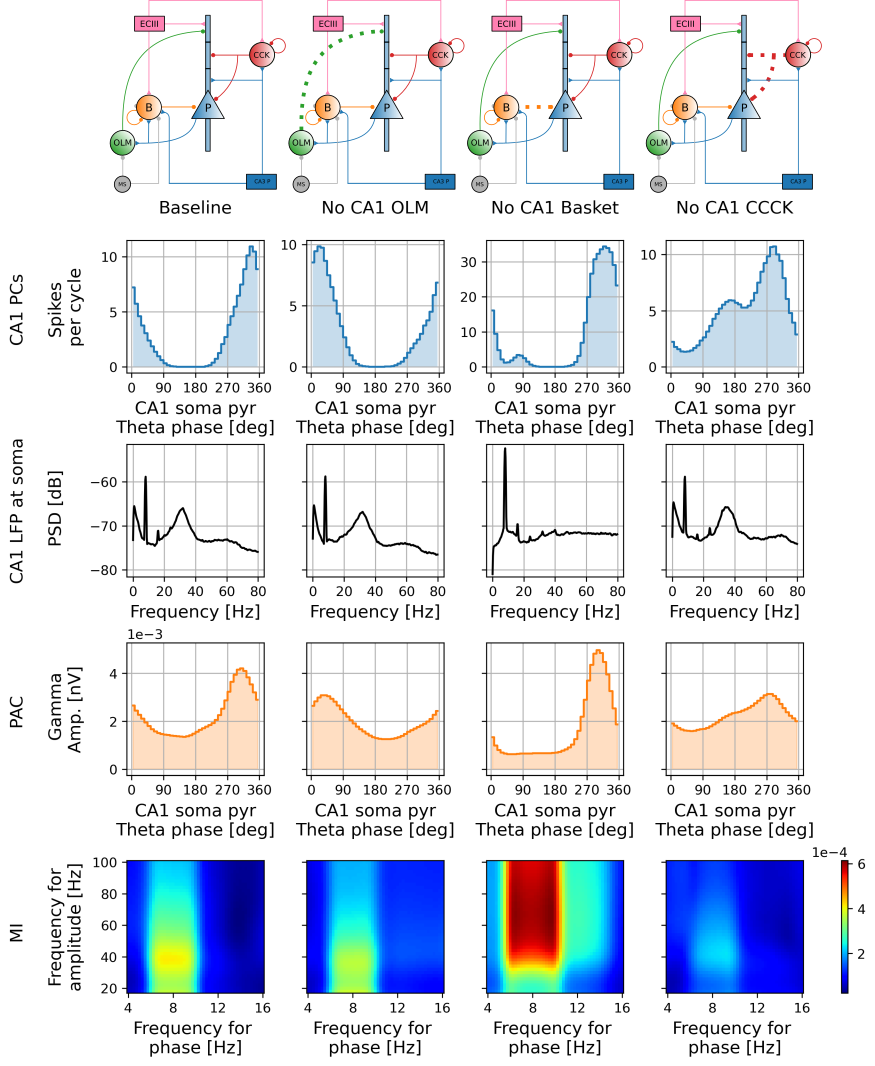
\includegraphics[width=\textwidth]{chapter4/figures/removing_interneurons/removing_interneurons_ca1_v2_lfp.png}
    \caption{\textbf{Effect of interneuron inhibition removal on CA1 subnetwork dynamics.}.
    From top to bottom: Distribution of spikes per theta cycle of pyramidal neurons, power spectral density  of the soma LFP, phase-amplitude coupling between theta and gamma filtered soma LFP, and modulation index of the soma LFP.
    From left to right: baseline state, removal of OLM cells projections, removal of basket cells projections, and removal of the CCK cells projections.
    Note that the scale is shared in each column excepting in the distribution plots.}
    \label{fig:no-inhibition-ca1-2}
\end{figure}
\begin{figure}[htbp]
    \ContinuedFloat % To indicate continuation of the previous table
    \centering
    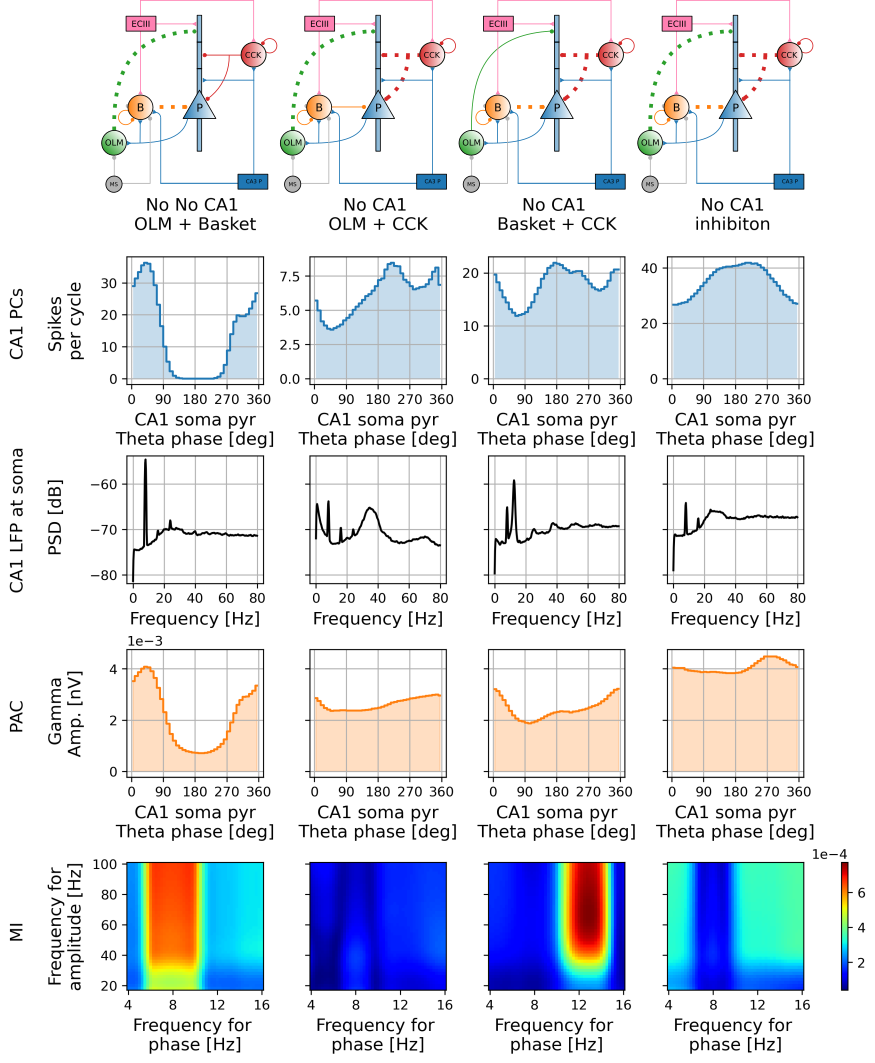
\includegraphics[width=\textwidth]{chapter4/figures/removing_interneurons/removing_interneurons_ca1_v3_lfp.png}
    \caption{\textbf{Effect of interneuron inhibition removal on CA1 subnetwork dynamics (continuation)}.
    From left to right: baseline state, removal of both OLM and basket cells projections, removal of both OLM and CKK cells projections, removal of both basket and CCK cells projections, and removal of all interneuron inhibition.}
    % \label{fig:no-inhibition-ca1-3}
\end{figure}
% rasters CA1 removing inhibition 2
\begin{figure}[htpb]
    \centering
    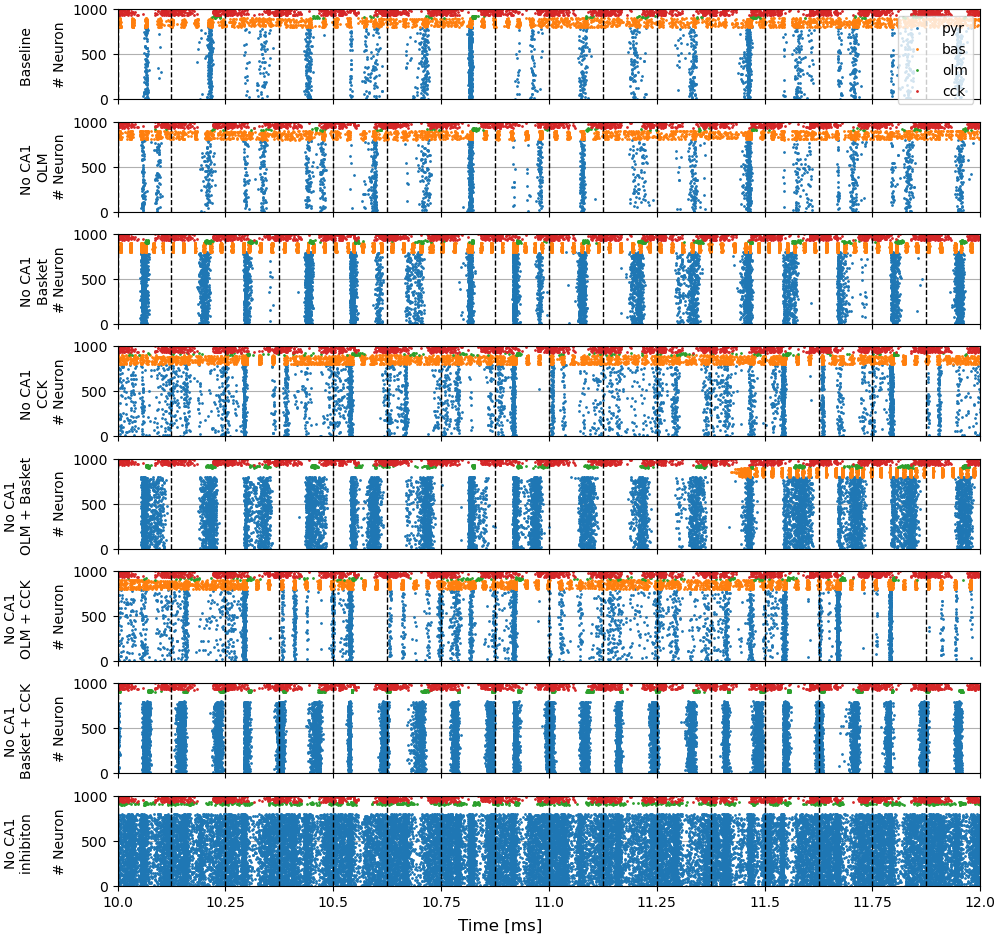
\includegraphics[width=\textwidth]{chapter4/figures/removing_interneurons/removing_interneurons_ca1_v4_rasters_new.png}
    \caption{\textbf{Effect of interneuron inhibition removal on CA1 subnetwork dynamics}.
    From top to bottom, the raster plots of the baseline state, the state of removing OLM cells projections, the state of removing basket cells projections, the state of removing CCK cells inhibition, the state of removing both OLM and basket cells projections, the state of removing both OLM and CCK cells projections, the state of removing both basketand CCK cells projections, and the state of removing all the inhibition.
    Blue, orange, green and red colors indicate pyramidal, basket OLM, and CCK cells, respectively.}
    \label{fig:interneurons-ca1-2-rasters}
\end{figure}
For completeness, we illustrate the scenario without inhibition from CCK cells, although we previously discussed their role in network dynamics in detail.
% Additionally, in Figure \ref{fig:no-inhibition-ca1-3}, we show the combined effects of removal various types of inhibition simultaneously.

% \textcolor{blue}{Figures \ref{a-fig:interneurons-ca3-lfps}, \ref{a-fig:interneurons-ca1-1-lfps}, \ref{a-fig:interneurons-ca1-2-lfps} and \ref{a-fig:interneurons-ca1-3-lfps} showcase theta- and gamma-filtered LFP measured at the soma stratum.}
\subsection{The role of synaptic inhibition in Basket cells in the generation and coupling of theta and gamma oscillations}
PV+ interneurons, including PV+ basket cells, play a crucial role as pacemakers and regulators of theta and gamma rhythms.
With their extensive connections, they have the capability to synchronize large networks of pyramidal cells, facilitating the coordinated firing patterns essential for these oscillations.
Synaptic inhibition directed towards PV+ interneurons serves as a fundamental mechanism in the generation of theta rhythms and the precise coupling of theta to gamma oscillations.
Any disruption in this inhibition leads to the breakdown of these rhythmic patterns, underscoring the intricately balanced regulation within neuronal networks \citep{wulff_hippocampal_2009}.

Electrophysiological recordings in awake, freely moving animals engaged in exploratory behavior have concluded signifcant conclusions.
Specifically, synaptic inhibition onto PV+ interneurons plays a substantial role in both the generation and modulation of theta and gamma oscillations.
Disruption of inhibitory control over PV+ interneurons leads to a decrease in the amplitude, frequency, and stability of theta oscillations.
Moreover, the absence of synaptic inhibition onto PV+ interneurons results in a disruption of the coupling between theta and gamma oscillations, consequently causing a reduction in the modulation of gamma oscillations by the theta phase \citep{wulff_hippocampal_2009}.

In our computational model, we conducted numerous experiments involving a systematic reduction of inhibition targeting basket cells.
This reduction was implemented in both the feedback inhibition and the inhibition of MS synthetic inputs.
We introduced a reduction factor, labeled as \textit{gain}, ranging from 0 to 1, which was applied to the conductances of the GABA$_\text{A}$ synapses involved in this process.
In Figure \ref{fig:CA1basket-deshibition}, we show the evolution of the amplitude and the stability (standard deviation) of the cycles of both theta and gamma components of the soma LFP as the parameter gain increases.
As mentioned earlier, the stability of the gamma component corresponds to the amplitude envelope.
Similarly, the evolution of the modulation index is presented.
\begin{figure}[!htb]
    \centering
    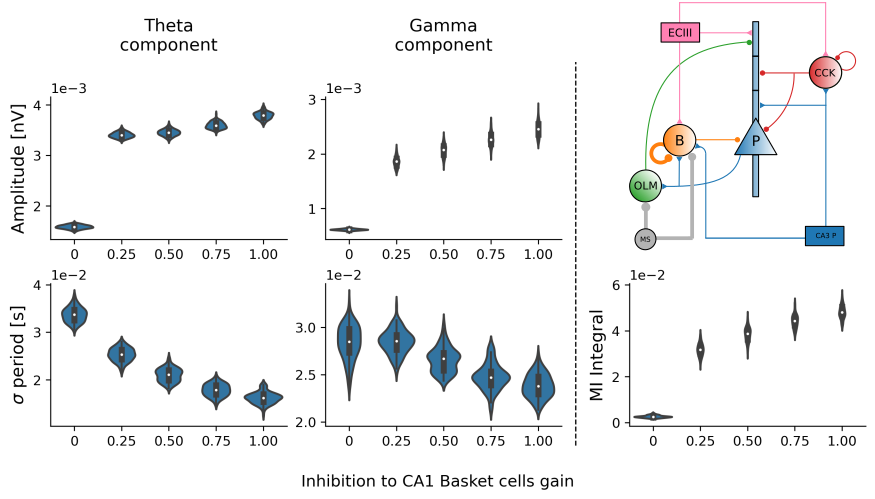
\includegraphics[width=\textwidth]{chapter4/figures/CA1basket_desinhibition.png}
    \caption{\textbf{Effect of inhibition to CA1 basket cells in the CA1 subnetwork dynamics}.
    Amplitude and standard deviation of theta and gamma oscillations (left), and the integral of the modulation index between theta and gamma as the GABAergic inhibition to CA1 basket cells is increased (right).
    Each violin corresponds to a distribution of 100 realizations.}
    \label{fig:CA1basket-deshibition}
\end{figure}
As the inhibition of basket cells is increased, the amplitude and the stability of theta and gamma oscillations increase, as well as the coupling between them, as observed in the modulation index.
Thus, inhibition into basket cells is crucial in the generation, enhancement, and stabilization of theta and gamma oscillations, as well as their coupling.

Therefore, the computational results align closely with the experimental observations, corroborating the pivotal role of synaptic inhibition in basket cells in the regulation of theta and gamma oscillations within the hippocampus.
However, contrary to the experimental findings, our model did not replicate variations in the frequency of theta oscillations. 
This aligns with our expectations, given that our model is driven by well-defined and stable theta sources. Consequently, the balance between these sources and the role of basket cells does not afford the latter enough influence to effect a significant variation in theta frequency.

% rasters CA1 removing inhibition 3
% \begin{figure}[htpb]
%     \centering
%     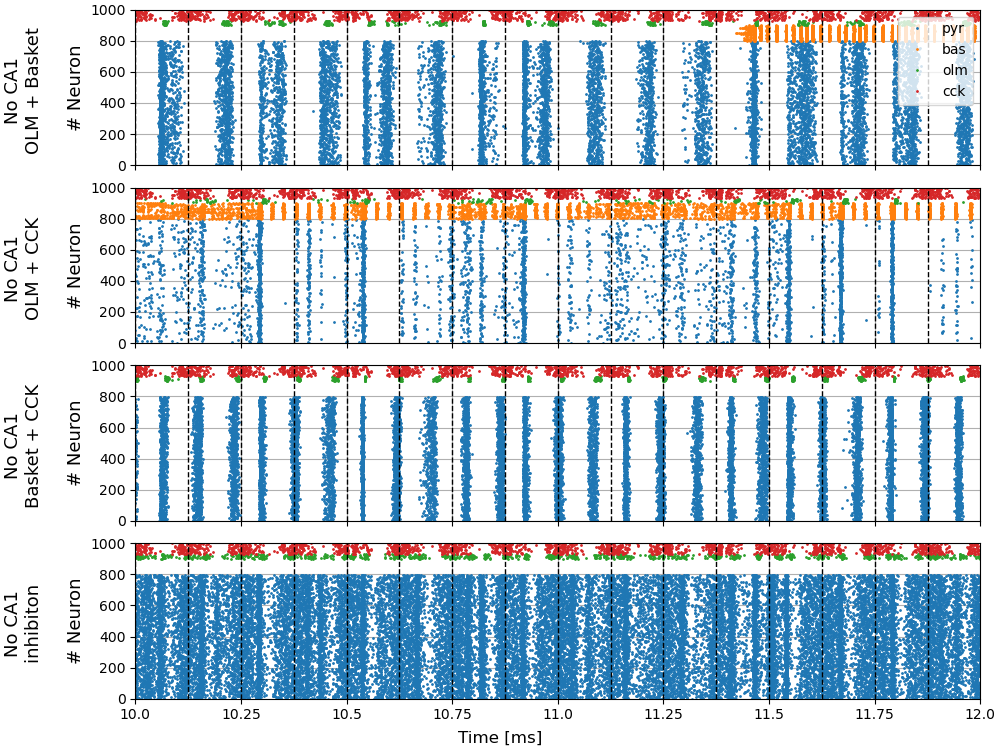
\includegraphics[width=\textwidth]{chapter4/figures/removing_interneurons/removing_interneurons_ca1_v3_rasters.png}
%     \caption{\textbf{Effect of interneuron inhibition removal on CA1 subnetwork dynamics (b)}.
%     From top to bottom, the raster plots of the baseline state, the state of removing both OLM and basket cells projections, the state of removing both OLM and CCK cells projections, the state of removing both basket and CKK cells projections, and the state of removing all interneuron inhibition.
%     Blue, orange, green and red colors indicate pyramidal, basket, and OLM cells, respectively.}
%     \label{a-fig:interneurons-ca1-3-rasters}
% \end{figure}

%%%%%%%%%%%%%%%%%%%%%%%%%%%%%%%%%%%%%%%%%%%%%%%%%%%%%%%%%%%%%%%%
% \subfile{../appendices/appendix3}
\end{document}

Compare results with results in \citep{wulff_hippocampal_2009}.
The authors performed several experiments to investigate the role of parvalbumin-positive (PV) interneurons and synaptic inhibition in the generation and coupling of theta and gamma oscillations in the hippocampus. 

1. Electrophysiological recordings: They recorded local field potentials (LFPs) and single-unit activity from the CA1 subfield of the hippocampus in control mice and PV-$\Delta\gamma$2 mice, which had synaptic inhibition onto PV interneurons disrupted. They analyzed various metrics, including theta amplitude, frequency, and cycle duration, as well as gamma amplitude, frequency, and modulation by theta phase.

2. Inhibitory postsynaptic currents (IPSCs): They recorded IPSCs in PV+ basket cells in brain slices from control and PV-$\Delta\gamma$2 mice. They compared the peak amplitudes and decay time constants of IPSCs between the two groups.

3. Computational modeling: They developed a computational model to simulate the network activity in the hippocampus with intact synaptic inhibition and with disrupted inhibition onto PV interneurons. They compared the network dynamics and oscillatory properties between the two models.

The animals were awake and freely moving during the electrophysiological recordings, and the experiments were conducted in both waking and paradoxical sleep (PS) states.

The main conclusions of the study are:

1. Synaptic inhibition onto PV interneurons is crucial for the generation and modulation of theta and gamma oscillations in the hippocampus.
2. Disruption of inhibitory control over PV interneurons leads to a reduction in theta oscillations, as evidenced by decreased amplitude, frequency, and stability of theta rhythm.
3. The coupling between theta and gamma oscillations is disrupted in the absence of synaptic inhibition onto PV interneurons, resulting in reduced modulation of gamma oscillations by theta phase.
4. Computational modeling supports the experimental findings, demonstrating that inhibitory connections onto PV interneurons are necessary for the generation and coupling of theta and gamma oscillations.

Citations: "IPSCs in the first group were characterized by large peak amplitudes ( 50 pA) and fast decay time constants ( 10 ms) and included all BCs recordings from control and 1 of 6 recordings from PV-$\Delta\gamma$2 BCs." "The PV-$\Delta\gamma$2 network

Recordings were performed during exploratory behavior (foraging
in an open field), awake immobility and sleep. 

%%%%%%%%%%%%%%%%%%%%%%%%%%%%%%%%%%%%%%%%%%%%%%%%%%%%%%%%%%%%%%%%%%%%%%%%%%%%%%%%%%%%%%

\subsection{Effect of CCK interneurons in CA1}
Poner aquello que hemos hecho para determinar la fase de las cck.


CCK interneurons (CCK-INs) in the CA1 region of the hippocampus have been shown to modulate the activity of CA1 pyramidal neurons . However, their role in gating cortical input-driven dendritic spikes (dSpikes) has not been investigated . In the study, the authors attempted to silence CCK-INs to understand their influence on LEC-driven dendritic activity in CA1 pyramidal neurons .

The authors tested three strategies to silence CCK-INs, including an intersectional approach to specifically target CCK-INs. However, none of these strategies successfully targeted or sufficiently hyperpolarized CCK-INs . Therefore, the silencing of CCK-INs was not possible at the time of the study .

The lack of successful silencing of CCK-INs prevented the authors from directly studying the effect of CCK-IN activity on LEC-driven dendritic activity. However, the authors did find that VIP interneurons (VIP-INs) serve a disinhibitory function to promote LEC-driven dSpike generation in CA1 pyramidal neurons . This suggests that VIP-INs play a role in modulating the activity of CA1 pyramidal neurons in response to cortical input.

In conclusion, while the authors were unable to directly investigate the effect of silencing CCK-INs, they demonstrated the involvement of VIP-INs in mediating disinhibition and promoting LEC-driven dSpike generation in CA1 pyramidal neurons . The study highlights the complex interplay between different types of interneurons and their role in regulating the activity of CA1 pyramidal neurons in response to cortical input. 

The recordings were performed using patch-clamp electrodes to measure the electrophysiological properties of CA1 neurons, such as firing and sag properties .

The animals were not actively engaged in any behavior during these measurements as they were in an anesthetized state. The purpose of these measurements was to investigate the intrinsic electrophysiological properties of CA1 neurons and their responses to various stimuli.

\citep{bilash_lateral_2023}


##### versión previa sobre el efecto de los inputs en ECII y en MS

The role of ECII and MS inputs.

To understand why this effect occurs, we need to delve into the details and analyze what is happening in each stratum.
The ECII inputs excite both the basket cells and the pyramidal at the Adend3 stratum, the distal dendrites.
Therefore, the net effect on basket cells is excitation since this input accelerates their firing, resulting in a frequency peak of 40 Hz in the gamma band.
When this input is removed, tha frequency decreases to 35 Hz.

On the other hand, within the pyramidal neuron, there is a filtering process from the distal dendrite to the soma, where they receive inhibition from basket cells.
Consequently, the basket-pyramidal interaction occurs with both elements being less excited, although the latter is less affected than the former compared to the baseline configuration.

En la Figura \ref{fig:no-ec2-input-ca3} mostramos una comparativa en los estratos del soma y de Adend3 entre el caso basal y el caso en el que los inputs de ECII se eliminan de la red. Para ello empleamos la LFP medida en ambos estratos y realizamos las medidas de PSD y MI sobre estas. Además, realizamos una medidas similares pero esta vez sobre las corrientes transmembrana en dichos estratos. 

En lo que respecta a la LFP, en ambos estratos, tanto el power en gamma como en theta se ven reducidos, a pesar de que el pico en theta aumenta, implicando que las oscilaciones theta son más constantes que en el caso basal.
En cuanto al cross-frequency coupling hemos distinguido dos medidas: el valor máximo y el valor de la integral sobre el espacio de frequencias theta-gamma.
Ambas medidas se ven reducidas significativamente en los dos estratos.

Sin embargo, la medida de la LFP se trata de una weighted sum de las aportaciones de cada estrato respecto al estrato donde se calcula. Por tanto, la LFP aunque capture principal el aporte de dicho estrato también están involucradas las aportaciones del resto de estratos.
Por tanto, una forma de eliminar estas aportanciones es tener en cuenta las corrientes transmembrana de dicho estrato, que es a partir de las cuales se determina la LFP.
Al realizar las mismas medidas, si que observamos diferencias. 
Mientras que en el estrato de Adend3, el power de la banda theta tiene el mismo efecto, en el estrato del soma el power aumenta.
Por tanto, el efecto de eliminar la excitación de las basket proveniente de los ECII inputs, y por tanto, que estas esten menos activas y reduciendo la frecuencia gamma dominante, da lugar a un aumento del power en theta. 

Del mismo modo que sucedía anteriormente, la amplitud del pico tanto en la banda gamma como en la theta aumentan.
En lo que respecta al modulation index, en el soma se observa un incremento tanto en la integral sobre el espacio de frecuencias de interés como en su máximo, mientras que en el estrato de Adend3, tiene lugar una reducción significativa del valor máximo, mientras que el valor de la integral no presenta un cambio significativo. 
Por tanto, este efecto de incremento del acoplamiento theta-gamma puede deberse a la interacción con la componente theta del estrato de Adend1, donde las piramidales reciben el input del giro dentado.



IF TIME ALLOWS 

\subsection{Effect of increase the CA3 PV+ basket cell}
Compare results with preeliminar results in \citep{lopez-madrona_different_2020}

Lo siguiente me lo ha dado Humata, pero debo asegurarme bien de lo que realmente pone en el paper:

In the initial experiments, the authors aimed to increase the activity of PV basket cells to investigate the independence of theta-gamma sources. They used optogenetic manipulation in behaving rats to selectively activate PV basket cells expressing ChR2 (channelrhodopsin-2). The rats were implanted with an electrode and two fibers, one for optogenetic stimulation and the other for recording local field potentials (LFPs). The rats were then trained in an open field and received ON/OFF periods of light stimulation to activate the PV basket cells.

The authors measured the LFPs in the hippocampus and prefrontal cortex to examine the theta-gamma coupling and synchronization between these regions. They analyzed the LFP data to assess the cross-frequency coupling (CFC) and theta synchronization between the two brain regions. They also compared the movement velocity of the rats between the novelty and habituation sessions as a control measure.

The results showed that during the novelty session, when the PV basket cells were activated, there was high theta synchronization and CFC between the hippocampus and prefrontal cortex. However, as the rats explored the familiar environment, the synchronization and CFC rapidly decayed in the known environment. By the end of the exploration time, both conditions reached the same level of theta synchronization, indicating that the introduced tactile stimulus had lost its novelty. The authors concluded that the theta-gamma coupling and synchronization between the hippocampus and prefrontal cortex are independent of PV basket cell activity and are influenced by the novelty of the environment.

Overall, the authors used optogenetic manipulation and LFP analysis to investigate the role of PV basket cells in theta-gamma coupling and synchronization between the hippocampus and prefrontal cortex. They demonstrated that the theta-gamma sources are independent of PV basket cell activity and are modulated by the novelty of the environment.